% Chapter 9: Seminar - Prophet and TBATS
% Quizzes, Practice Problems, and Discussion
% Bachelor program, Bucharest University of Economic Studies

\documentclass[9pt, aspectratio=169, t]{beamer}

% Ensure content fits on slides
\setbeamersize{text margin left=8mm, text margin right=8mm}

%=============================================================================
% THEME AND STYLE CONFIGURATION
%=============================================================================
\usetheme{default}
% Using default theme for clean header/footer control

% Color Palette (matching Redispatch PDF)
\definecolor{MainBlue}{RGB}{26, 58, 110}
\definecolor{AccentBlue}{RGB}{26, 58, 110}
\definecolor{IDAred}{RGB}{205, 0, 0}
\definecolor{DarkGray}{RGB}{51, 51, 51}
\definecolor{MediumGray}{RGB}{128, 128, 128}
\definecolor{LightGray}{RGB}{248, 248, 248}
\definecolor{VeryLightGray}{RGB}{235, 235, 235}
\definecolor{KeynoteGray}{RGB}{218, 218, 218}
\definecolor{SectionGray}{RGB}{120, 120, 120}
\definecolor{FooterGray}{RGB}{100, 100, 100}
\definecolor{Crimson}{RGB}{220, 53, 69}
\definecolor{Forest}{RGB}{46, 125, 50}
\definecolor{Amber}{RGB}{181, 133, 63}
\definecolor{Orange}{RGB}{230, 126, 34}
\definecolor{Purple}{RGB}{142, 68, 173}

% Gradient background (exact Keynote 315° gradient: white to RGB 218,218,218)
\setbeamertemplate{background}{%
    \begin{tikzpicture}[remember picture, overlay]
        \shade[shading=axis, shading angle=315,
        top color=white, bottom color=KeynoteGray]
        (current page.south west) rectangle (current page.north east);
    \end{tikzpicture}%
}
% Fallback solid color for compatibility
\setbeamercolor{background canvas}{bg=}

\setbeamercolor{palette primary}{bg=MainBlue, fg=white}
\setbeamercolor{palette secondary}{bg=MainBlue!85, fg=white}
\setbeamercolor{palette tertiary}{bg=MainBlue!70, fg=white}
\setbeamercolor{structure}{fg=MainBlue}
\setbeamercolor{title}{fg=IDAred}
\setbeamercolor{frametitle}{fg=IDAred, bg=}
\setbeamercolor{block title}{bg=MainBlue, fg=white}
\setbeamercolor{block body}{bg=VeryLightGray, fg=DarkGray}
\setbeamercolor{block title alerted}{bg=Crimson, fg=white}
\setbeamercolor{block body alerted}{bg=Crimson!8, fg=DarkGray}
\setbeamercolor{block title example}{bg=Forest, fg=white}
\setbeamercolor{block body example}{bg=Forest!8, fg=DarkGray}
\setbeamercolor{item}{fg=MainBlue}

% Footer colors (override Madrid theme blue)
\setbeamercolor{author in head/foot}{fg=FooterGray, bg=}
\setbeamercolor{title in head/foot}{fg=FooterGray, bg=}
\setbeamercolor{date in head/foot}{fg=FooterGray, bg=}
\setbeamercolor{section in head/foot}{fg=FooterGray, bg=}
\setbeamercolor{subsection in head/foot}{fg=FooterGray, bg=}

% Bullet styles (apply everywhere including blocks)
\setbeamertemplate{itemize item}{\color{MainBlue}$\boxdot$}
\setbeamertemplate{itemize subitem}{\color{MainBlue}$\blacktriangleright$}
\setbeamertemplate{itemize subsubitem}{\color{MainBlue}\tiny$\bullet$}
\setbeamertemplate{itemize/enumerate body begin}{\normalsize}
\setbeamertemplate{itemize/enumerate subbody begin}{\normalsize}

% Item spacing - compact style
\setlength{\leftmargini}{10pt}       % Level 1: minimal indent
\setlength{\leftmarginii}{10pt}      % Level 2: minimal additional indent
% Compact list spacing (zero extra space before/after lists in blocks)
\makeatletter
\def\@listi{\leftmargin\leftmargini \topsep 0pt \parsep 0pt \itemsep 0pt}
\def\@listii{\leftmargin\leftmarginii \topsep 0pt \parsep 0pt \itemsep 0pt}
\makeatother

\setbeamertemplate{navigation symbols}{}

%=============================================================================
% CUSTOM HEADLINE
%=============================================================================
\setbeamertemplate{headline}{%
    \vskip10pt%
    \hbox to \paperwidth{%
        \hskip0.5cm%
        {\small\color{FooterGray}\renewcommand{\hyperlink}[2]{##2}\insertsectionhead}%
        \hfill%
        \textcolor{FooterGray}{\small\insertframenumber}%
        \hskip0.5cm%
    }%
    \vskip4pt%
    {\color{FooterGray}\hrule height 0.4pt}%
}

%=============================================================================
% CUSTOM FOOTER
%=============================================================================
\usepackage{fontawesome5}

\setbeamertemplate{footline}{%
    {\color{FooterGray}\hrule height 0.4pt}%
    \vskip4pt%
    \hbox to \paperwidth{%
        \hskip0.5cm%
        \textcolor{FooterGray}{\small Time Series Analysis and Forecasting}%
        \hfill%
        \raisebox{-0.1em}{%
            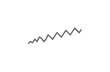
\begin{tikzpicture}[x=0.08em, y=0.08em, line width=0.4pt]
                \draw[FooterGray] (0,3) -- (1,4) -- (2,3.5) -- (3,5) -- (4,4) -- (5,6) -- (6,5.5) -- (7,4) -- (8,5) -- (9,7) -- (10,6) -- (11,5) -- (12,6.5) -- (13,8) -- (14,7) -- (15,6) -- (16,7.5) -- (17,9) -- (18,8) -- (19,7) -- (20,8.5) -- (21,10) -- (22,9) -- (23,8) -- (24,9.5);
            \end{tikzpicture}%
        }%
        \hskip0.5cm%
    }%
    \vskip6pt%
}

%=============================================================================
% PACKAGES
%=============================================================================
\usepackage[utf8]{inputenc}
\usepackage[T1]{fontenc}
\usepackage[english]{babel}
\usepackage{amsmath, amssymb, amsthm}
\usepackage{mathtools}
\usepackage{bm}
\usepackage{tikz}
\usetikzlibrary{arrows.meta, positioning, shapes, calc, decorations.pathreplacing, shadings}
\usepackage{booktabs}
\usepackage{multirow}
\usepackage{array}
\usepackage{graphicx}
\usepackage{hyperref}
\usepackage{colortbl}
\hypersetup{colorlinks=true, linkcolor=MainBlue, urlcolor=MainBlue}
\graphicspath{{../../logos/}{../../charts/}}
\hfuzz=2pt  % Suppress tiny overfull warnings (<2pt)
\vfuzz=2pt  % Suppress tiny vertical overfull warnings (<2pt)

%=============================================================================
% QUANTLET COMMAND
%=============================================================================
\newcommand{\quantlet}[2]{%
    \hfill\href{#2}{%
        \raisebox{-0.15em}{\includegraphics[height=0.7em]{ql_logo.png}}%
        \textcolor{MainBlue}{\tiny\ #1}%
    }%
}

%=============================================================================
% CUSTOM COMMANDS
%=============================================================================
\newcommand{\E}{\mathbb{E}}
\newcommand{\Var}{\text{Var}}
\newcommand{\Cov}{\text{Cov}}

%=============================================================================
% TITLE INFORMATION
%=============================================================================
\title[Chapter 9: Seminar]{Chapter 9: Seminar --- Prophet \& TBATS}
\subtitle{Bachelor program Faculty of Cybernetics, Statistics and Economic Informatics, Bucharest University of Economic Studies, Romania}
\author[Prof. dr. Daniel Traian Pele]{Prof. dr. Daniel Traian Pele\\[0.2cm]\footnotesize\texttt{danpele@ase.ro}}
\institute{Bucharest University of Economic Studies}
\date{Academic Year 2025--2026}

\begin{document}

%=============================================================================
% TITLE SLIDE
%=============================================================================
\begin{frame}[plain]
    \begin{tikzpicture}[remember picture, overlay]
        \fill[IDAred] (current page.north west) rectangle ([yshift=-0.15cm]current page.north east);
        \node[anchor=north west] at ([xshift=0.5cm, yshift=-0.3cm]current page.north west) {
            \href{https://www.ase.ro}{\includegraphics[height=1.1cm]{ase_logo.png}}
        };
        \node[anchor=north] at ([yshift=-0.3cm]current page.north) {
            \href{https://ai4efin.ase.ro}{\includegraphics[height=1.1cm]{ai4efin_logo.png}}
        };
        \node[anchor=north east] at ([xshift=-0.5cm, yshift=-0.3cm]current page.north east) {
            \href{https://www.digital-finance-msca.com}{\includegraphics[height=1.1cm]{msca_logo.png}}
        };
    \end{tikzpicture}
    \vfill
    \begin{center}
        {\Large\textcolor{MediumGray}{Time Series Analysis and Forecasting}}\\[0.3cm]
        {\Huge\textbf{\textcolor{MainBlue}{Chapter 9: Prophet \& TBATS}}}\\[0.5cm]
        {\Large\textcolor{IDAred}{Seminar}}
    \end{center}
    \vfill

    \begin{tikzpicture}[remember picture, overlay]
        \fill[IDAred] (current page.south west) rectangle ([yshift=0.15cm]current page.south east);
        \node[anchor=south west] at ([xshift=0.5cm, yshift=0.8cm]current page.south west) {
            \href{https://theida.net}{\includegraphics[height=0.9cm]{ida_logo.png}}
        };
        \node[anchor=south] at ([xshift=-3cm, yshift=0.8cm]current page.south) {
            \href{https://blockchain-research-center.com}{\includegraphics[height=0.9cm]{brc_logo.png}}
        };
        \node[anchor=south] at ([yshift=0.8cm]current page.south) {
            \href{https://quantinar.com}{\includegraphics[height=0.9cm]{qr_logo.png}}
        };
        \node[anchor=south] at ([xshift=3cm, yshift=0.8cm]current page.south) {
            \href{https://quantlet.com}{\includegraphics[height=0.9cm]{ql_logo.png}}
        };
        \node[anchor=south east] at ([xshift=-0.5cm, yshift=0.8cm]current page.south east) {
            \href{https://ipe.ro/new}{\includegraphics[height=0.9cm]{acad_logo.png}}
        };
    \end{tikzpicture}
\end{frame}

%=============================================================================
% OUTLINE
%=============================================================================
\begin{frame}{Seminar Outline}
    \tableofcontents
\end{frame}

%=============================================================================
% SECTION 1: REVIEW QUIZ
%=============================================================================
\section{Review Quiz}

\begin{frame}{Quiz 1: Multiple Seasonality Challenge}
    \begin{alertblock}{Question}
        Why can't standard SARIMA handle hourly electricity demand data?
    \end{alertblock}

    \vspace{0.3cm}

    \begin{enumerate}[A)]
        \item SARIMA can only handle monthly data
        \item SARIMA allows only one seasonal period ($m$ parameter)
        \item SARIMA doesn't support trend components
        \item SARIMA requires normally distributed data
    \end{enumerate}

    \vspace{0.5cm}
    \begin{flushright}\textit{Answer on next slide...}\end{flushright}
\end{frame}

\begin{frame}{Quiz 1: Answer}
    \begin{exampleblock}{Answer: B -- SARIMA allows only one seasonal period}
        \begin{center}
            \includegraphics[width=0.85\textwidth, height=0.60\textheight, keepaspectratio]{ch9_quiz1_multiple_seasonality.pdf}
        \end{center}
        \vspace{-0.2cm}
        {\footnotesize
        \textbf{Key}: Hourly data has daily (24h), weekly (168h), and annual (8760h) patterns. SARIMA's single $m$ parameter cannot capture all these simultaneously.
        }
    \end{exampleblock}
\end{frame}

\begin{frame}{Quiz 2: TBATS Acronym}
    \begin{alertblock}{Question}
        What does TBATS stand for?
    \end{alertblock}

    \vspace{0.3cm}

    \begin{enumerate}[A)]
        \item Trend, Baseline, ARMA, Transform, Seasonal
        \item Trigonometric, Box-Cox, ARMA, Trend, Seasonal
        \item Time-Based Automatic Time Series
        \item Temporal Bayesian Adaptive Trend System
    \end{enumerate}

    \vspace{0.5cm}
    \begin{flushright}\textit{Answer on next slide...}\end{flushright}
\end{frame}

\begin{frame}{Quiz 2: Answer}
    \begin{exampleblock}{Answer: B -- Trigonometric, Box-Cox, ARMA, Trend, Seasonal}
        \begin{center}
            \includegraphics[width=0.85\textwidth, height=0.48\textheight, keepaspectratio]{ch9_quiz2_tbats_components.pdf}
        \end{center}
        \vspace{-0.3cm}
        {\scriptsize
        \textbf{TBATS}: \textbf{T}rigonometric (Fourier for seasonality), \textbf{B}ox-Cox (variance stabilization), \textbf{A}RMA (error autocorrelation), \textbf{T}rend (damped local), \textbf{S}easonal (multiple periods).
        }
    \end{exampleblock}
\end{frame}

\begin{frame}{Quiz 3: Fourier Terms}
    \begin{alertblock}{Question}
        In TBATS, increasing the number of Fourier harmonics ($K$) for a seasonal pattern:
    \end{alertblock}

    \vspace{0.3cm}

    \begin{enumerate}[A)]
        \item Always improves forecast accuracy
        \item Allows more flexible (complex) seasonal shapes
        \item Reduces the model complexity
        \item Eliminates the need for Box-Cox transformation
    \end{enumerate}

    \vspace{0.5cm}
    \begin{flushright}\textit{Answer on next slide...}\end{flushright}
\end{frame}

\begin{frame}{Quiz 3: Answer}
    \begin{exampleblock}{Answer: B -- Allows more flexible seasonal shapes}
        \begin{center}
            \includegraphics[width=0.85\textwidth, height=0.51\textheight, keepaspectratio]{ch9_quiz3_fourier_harmonics.pdf}
        \end{center}
        \vspace{-0.2cm}
        {\footnotesize
        \textbf{Trade-off}: More harmonics = more flexibility but also more parameters.
        $$s_t^{(i)} = \sum_{j=1}^{K_i} \left[ a_j^{(i)} \cos\left(\frac{2\pi j t}{m_i}\right) + b_j^{(i)} \sin\left(\frac{2\pi j t}{m_i}\right) \right]$$
        }
    \end{exampleblock}
\end{frame}

\begin{frame}{Quiz 4: Prophet Decomposition}
    \begin{alertblock}{Question}
        Prophet decomposes a time series into which components?
    \end{alertblock}

    \vspace{0.3cm}

    \begin{enumerate}[A)]
        \item AR, MA, and seasonal components
        \item Trend, seasonality, holidays, and error
        \item Mean, variance, and autocorrelation
        \item Level, slope, and curvature
    \end{enumerate}

    \vspace{0.5cm}
    \begin{flushright}\textit{Answer on next slide...}\end{flushright}
\end{frame}

\begin{frame}{Quiz 4: Answer}
    \begin{exampleblock}{Answer: B -- Trend, seasonality, holidays, and error}
        \begin{center}
            \includegraphics[width=0.85\textwidth, height=0.50\textheight, keepaspectratio]{ch9_quiz4_prophet_decomposition.pdf}
        \end{center}
        \vspace{-0.3cm}
        {\scriptsize
        \textbf{Prophet}: $y(t) = g(t) + s(t) + h(t) + \varepsilon_t$ where $g(t)$ = trend, $s(t)$ = seasonality (Fourier), $h(t)$ = holidays, $\varepsilon_t$ = error.
        }
    \end{exampleblock}
\end{frame}

\begin{frame}{Quiz 5: Prophet vs TBATS}
    \begin{alertblock}{Question}
        When would you choose Prophet over TBATS?
    \end{alertblock}

    \vspace{0.3cm}

    \begin{enumerate}[A)]
        \item When you need automatic model selection
        \item When you have known holidays and changepoints to incorporate
        \item When you need the most parsimonious model
        \item When your data has no trend
    \end{enumerate}

    \vspace{0.5cm}
    \begin{flushright}\textit{Answer on next slide...}\end{flushright}
\end{frame}

\begin{frame}{Quiz 5: Answer}
    \begin{exampleblock}{Answer: B -- Known holidays and changepoints}
        \begin{center}
            \includegraphics[width=0.85\textwidth, height=0.58\textheight, keepaspectratio]{ch9_quiz5_prophet_vs_tbats.pdf}
        \end{center}
        \vspace{-0.2cm}
        {\footnotesize
        \textbf{Prophet advantages}: Easy holiday integration, analyst-in-the-loop, handles missing data, interpretable components. \\
        \textbf{TBATS advantages}: Automatic model selection, handles complex seasonality without domain expertise.
        }
    \end{exampleblock}
\end{frame}

\begin{frame}{Quiz 6: Seasonality Mode}
    \begin{alertblock}{Question}
        For retail sales data where December sales are 3x the monthly average, which seasonality mode is more appropriate in Prophet?
    \end{alertblock}

    \vspace{0.3cm}

    \begin{enumerate}[A)]
        \item Additive seasonality
        \item Multiplicative seasonality
        \item Both work equally well
        \item Neither---use ARIMA instead
    \end{enumerate}

    \vspace{0.5cm}
    \begin{flushright}\textit{Answer on next slide...}\end{flushright}
\end{frame}

\begin{frame}{Quiz 6: Answer}
    \begin{exampleblock}{Answer: B -- Multiplicative seasonality}
        \begin{center}
            \includegraphics[width=0.85\textwidth, height=0.58\textheight, keepaspectratio]{ch9_quiz6_seasonality_mode.pdf}
        \end{center}
        \vspace{-0.2cm}
        {\footnotesize
        \textbf{Key}: When seasonal amplitude scales with the level, use multiplicative. \\
        \textbf{Additive}: $y = g(t) + s(t)$ (constant seasonal effect) \\
        \textbf{Multiplicative}: $y = g(t) \cdot (1 + s(t))$ (proportional seasonal effect)
        }
    \end{exampleblock}
\end{frame}

\begin{frame}{Quiz 7: Prophet Changepoints}
    \begin{alertblock}{Question}
        In Prophet, changepoints allow the model to:
    \end{alertblock}

    \vspace{0.3cm}

    \begin{enumerate}[A)]
        \item Change the seasonal period automatically
        \item Adjust the trend slope at specific points in time
        \item Switch between additive and multiplicative modes
        \item Detect and remove outliers
    \end{enumerate}

    \vspace{0.5cm}
    \begin{flushright}\textit{Answer on next slide...}\end{flushright}
\end{frame}

\begin{frame}{Quiz 7: Answer}
    \begin{exampleblock}{Answer: B -- Adjust trend slope at specific points}
        \begin{center}
            \includegraphics[width=0.85\textwidth, height=0.53\textheight, keepaspectratio]{ch9_quiz7_changepoints.pdf}
        \end{center}
        \vspace{-0.2cm}
        {\footnotesize
        \textbf{Changepoints}: Allow piecewise linear trend with different slopes.
        $$g(t) = (k + \mathbf{a}(t)^\top \boldsymbol{\delta}) \cdot t + (m + \mathbf{a}(t)^\top \boldsymbol{\gamma})$$
        Prophet automatically detects changepoints or you can specify them manually.
        }
    \end{exampleblock}
\end{frame}

\begin{frame}{Quiz 8: Model Selection}
    \begin{alertblock}{Question}
        You have daily call center data with weekly seasonality only. Which model is most appropriate?
    \end{alertblock}

    \vspace{0.3cm}

    \begin{enumerate}[A)]
        \item TBATS (designed for multiple seasonality)
        \item Prophet (handles any seasonality well)
        \item Standard SARIMA (simpler and sufficient)
        \item LSTM neural network (most flexible)
    \end{enumerate}

    \vspace{0.5cm}
    \begin{flushright}\textit{Answer on next slide...}\end{flushright}
\end{frame}

\begin{frame}{Quiz 8: Answer}
    \begin{exampleblock}{Answer: C -- Standard SARIMA is sufficient}
        \begin{center}
            \includegraphics[width=0.85\textwidth, height=0.58\textheight, keepaspectratio]{ch9_quiz8_model_decision.pdf}
        \end{center}
        \vspace{-0.2cm}
        {\footnotesize
        \textbf{Principle of parsimony}: Use the simplest model that fits the data. \\
        With only weekly seasonality ($m=7$), SARIMA works fine. \\
        Use TBATS/Prophet when you \textit{need} multiple seasonalities or special features.
        }
    \end{exampleblock}
\end{frame}

\begin{frame}{Quiz 9: Prophet Uncertainty}
    \begin{alertblock}{Question}
        Prophet generates prediction intervals by:
    \end{alertblock}

    \vspace{0.3cm}

    \begin{enumerate}[A)]
        \item Assuming normally distributed residuals
        \item Sampling from the posterior distribution of parameters
        \item Using bootstrap resampling of historical errors
        \item Applying a fixed multiplier to point forecasts
    \end{enumerate}

    \vspace{0.5cm}
    \begin{flushright}\textit{Answer on next slide...}\end{flushright}
\end{frame}

\begin{frame}{Quiz 9: Answer}
    \begin{exampleblock}{Answer: B -- Sampling from posterior distribution}
        \begin{center}
            \includegraphics[width=0.85\textwidth, height=0.52\textheight, keepaspectratio]{ch9_quiz9_prophet_uncertainty.pdf}
        \end{center}
        \vspace{-0.3cm}
        {\scriptsize
        \textbf{Prophet uses Bayesian estimation}: MAP for point forecasts, MCMC/simulation for intervals. Uncertainty from both trend (changepoints) and observation noise.
        }
    \end{exampleblock}
\end{frame}

\begin{frame}{Quiz 10: Practical Application}
    \begin{alertblock}{Question}
        For forecasting hourly energy demand with daily, weekly, and annual patterns plus holiday effects, which approach is best?
    \end{alertblock}

    \vspace{0.3cm}

    \begin{enumerate}[A)]
        \item SARIMA with $m=24$
        \item TBATS with three seasonal periods
        \item Prophet with custom holidays
        \item Either TBATS or Prophet, depending on whether holidays are important
    \end{enumerate}

    \vspace{0.5cm}
    \begin{flushright}\textit{Answer on next slide...}\end{flushright}
\end{frame}

\begin{frame}{Quiz 10: Answer}
    \begin{exampleblock}{Answer: D -- TBATS or Prophet depending on needs}
        \begin{center}
            \includegraphics[width=0.85\textwidth, height=0.52\textheight, keepaspectratio]{ch9_quiz10_energy_example.pdf}
        \end{center}
        \vspace{-0.3cm}
        {\scriptsize
        \textbf{Both handle multiple seasonality}: Holiday effects crucial $\Rightarrow$ Prophet; automatic selection $\Rightarrow$ TBATS. Often try both and compare via cross-validation.
        }
    \end{exampleblock}
\end{frame}

%=============================================================================
% TRUE/FALSE QUESTIONS
%=============================================================================
\section{True/False Questions}

\begin{frame}{True/False Questions}
    Determine if each statement is True or False:

    \vspace{0.3cm}
    \begin{enumerate}
        \item Prophet was developed by Facebook (Meta) for business forecasting.
        \item TBATS can only handle two seasonal periods at most.
        \item In Prophet, the default trend is logistic growth.
        \item Fourier terms approximate seasonality using sine and cosine functions.
        \item Prophet requires equally spaced time series data.
        \item The Box-Cox transformation in TBATS stabilizes variance.
    \end{enumerate}

    \vspace{0.3cm}
    \begin{flushright}\textit{Answers on next slide...}\end{flushright}
\end{frame}

\begin{frame}{True/False: Solutions}
    {\small
    \begin{enumerate}\setlength{\itemsep}{1pt}
        \item Prophet was developed by Facebook (Meta) for business forecasting. \hfill \textcolor{Forest}{\textbf{TRUE}}

        {\footnotesize \textcolor{MediumGray}{Released in 2017, designed for ``analyst in the loop'' forecasting at scale.}}

        \item TBATS can only handle two seasonal periods at most. \hfill \textcolor{Crimson}{\textbf{FALSE}}

        {\footnotesize \textcolor{MediumGray}{TBATS can handle any number of seasonal periods (e.g., daily, weekly, annual).}}

        \item In Prophet, the default trend is logistic growth. \hfill \textcolor{Crimson}{\textbf{FALSE}}

        {\footnotesize \textcolor{MediumGray}{Default is piecewise linear. Logistic growth must be explicitly specified.}}

        \item Fourier terms approximate seasonality using sine and cosine functions. \hfill \textcolor{Forest}{\textbf{TRUE}}

        {\footnotesize \textcolor{MediumGray}{$s(t) = \sum_{k=1}^{K}[a_k \cos(2\pi kt/m) + b_k \sin(2\pi kt/m)]$}}

        \item Prophet requires equally spaced time series data. \hfill \textcolor{Crimson}{\textbf{FALSE}}

        {\footnotesize \textcolor{MediumGray}{Prophet handles missing data and irregular timestamps gracefully.}}

        \item The Box-Cox transformation in TBATS stabilizes variance. \hfill \textcolor{Forest}{\textbf{TRUE}}

        {\footnotesize \textcolor{MediumGray}{$y^{(\lambda)} = (y^\lambda - 1)/\lambda$ for $\lambda \neq 0$; $\log(y)$ for $\lambda = 0$.}}
    \end{enumerate}
    }
\end{frame}

%=============================================================================
% KEY DEFINITIONS
%=============================================================================
\section{Key Definitions}

\begin{frame}{Fourier Series Representation}
    \begin{block}{Definition: Fourier Harmonics}
        A \textbf{Fourier series} represents a periodic function $s(t)$ with period $m$ as:
        \[
        s(t) = a_0 + \sum_{k=1}^{K} \left[ a_k \cos\left(\frac{2\pi k t}{m}\right) + b_k \sin\left(\frac{2\pi k t}{m}\right) \right]
        \]
        where:
        \begin{itemize}
            \item $k$: harmonic number (frequency multiplier)
            \item $a_k, b_k$: Fourier coefficients (estimated from data)
            \item $K$: number of harmonics (controls flexibility)
        \end{itemize}
    \end{block}

    \begin{exampleblock}{Why It Works}
        \textbf{Fourier's Theorem}: Any periodic function can be expressed as a (possibly infinite) sum of sine and cosine waves. With finite $K$, we get an approximation.
    \end{exampleblock}
\end{frame}

%=============================================================================
% SECTION 2: PRACTICE PROBLEMS
%=============================================================================
\section{Practice Problems}

\begin{frame}{Problem 1: Fourier Terms Calculation}
    \begin{block}{Exercise}
        For daily data with weekly seasonality ($m=7$), you want to use Fourier terms with $K=3$ harmonics.

        \vspace{0.2cm}
        How many parameters does this add to the model?
    \end{block}

    \vspace{0.5cm}
    \begin{flushright}\textit{Answer on next slide...}\end{flushright}
\end{frame}

\begin{frame}[fragile]{Problem 1: Solution}
    \vspace{-0.6cm}
    \begin{exampleblock}{Solution: 6 parameters}
        \textbf{Each harmonic} requires 2 parameters (sine and cosine coefficients):
        $$s(t) = \sum_{k=1}^{K} \left[ a_k \cos\left(\frac{2\pi k t}{m}\right) + b_k \sin\left(\frac{2\pi k t}{m}\right) \right]$$

        \vspace{0.1cm}
        With $K=3$ harmonics:
        \begin{itemize}
            \item $k=1$: $a_1, b_1$ (fundamental frequency $1/7$ cycles per day)
            \item $k=2$: $a_2, b_2$ (first overtone, $2/7$ cycles per day)
            \item $k=3$: $a_3, b_3$ (second overtone, $3/7$ cycles per day)
        \end{itemize}

        \vspace{0.1cm}
        \textbf{Total}: $2 \times K = 2 \times 3 = 6$ parameters
    \end{exampleblock}

    \begin{alertblock}{Nyquist Limit}
        Maximum useful $K = \lfloor m/2 \rfloor$. With $m$ discrete observations per period, we can identify at most $m/2$ distinct frequencies. For $m=7$: $K_{\max} = 3$.
    \end{alertblock}
\end{frame}

\begin{frame}{Problem 2: Choosing Seasonality Mode}
    \begin{block}{Exercise}
        You're forecasting monthly hotel bookings. The data shows:
        \begin{itemize}
            \item July 2020: 1000 bookings (peak season)
            \item January 2020: 400 bookings (off-season)
            \item July 2023: 2000 bookings (peak season)
            \item January 2023: 800 bookings (off-season)
        \end{itemize}

        Should you use additive or multiplicative seasonality? Why?
    \end{block}

    \vspace{0.5cm}
    \begin{flushright}\textit{Answer on next slide...}\end{flushright}
\end{frame}

\begin{frame}[fragile]{Problem 2: Solution}
    \begin{exampleblock}{Solution: Multiplicative seasonality}
        \textbf{Analysis}: Check if seasonal amplitude is proportional to level.

        \vspace{0.2cm}
        \begin{tabular}{lccc}
            \toprule
            Year & July & January & Ratio (Jul/Jan) \\
            \midrule
            2020 & 1000 & 400 & 2.5 \\
            2023 & 2000 & 800 & 2.5 \\
            \bottomrule
        \end{tabular}

        \vspace{0.3cm}
        \textbf{Key observation}: The \textit{ratio} stays constant (2.5), not the difference!
        \begin{itemize}
            \item Additive would mean: July always +600 above January
            \item But 2020: $1000 - 400 = 600$; 2023: $2000 - 800 = 1200$
        \end{itemize}

        \vspace{0.2cm}
        \textbf{Conclusion}: Use multiplicative: \texttt{seasonality\_mode='multiplicative'}
    \end{exampleblock}
\end{frame}

\begin{frame}{Problem 3: TBATS Model Interpretation}
    \begin{block}{Exercise}
        A TBATS model fitted to hourly electricity data reports:
        \begin{itemize}
            \item Box-Cox $\lambda = 0.5$
            \item Seasonal periods: $m_1 = 24$, $m_2 = 168$
            \item Fourier terms: $K_1 = 5$, $K_2 = 3$
        \end{itemize}

        What does each component tell you about the data?
    \end{block}

    \vspace{0.5cm}
    \begin{flushright}\textit{Answer on next slide...}\end{flushright}
\end{frame}

\begin{frame}[fragile]{Problem 3: Solution}
    \vspace{-0.3cm}
    \begin{exampleblock}{Solution}
        \textbf{Box-Cox $\lambda = 0.5$}:
        \begin{itemize}
            \item Square root transformation applied
            \item Data had increasing variance with level
            \item Transformation: $y^{(0.5)} = \sqrt{y}$
        \end{itemize}

        \vspace{0.2cm}
        \textbf{Seasonal periods}:
        \begin{itemize}
            \item $m_1 = 24$: Daily pattern (24 hours)
            \item $m_2 = 168$: Weekly pattern ($7 \times 24 = 168$ hours)
        \end{itemize}

        \vspace{0.2cm}
        \textbf{Fourier terms}:
        \begin{itemize}
            \item $K_1 = 5$ for daily: Complex intraday pattern (5 harmonics capture peaks, valleys)
            \item $K_2 = 3$ for weekly: Simpler weekly pattern (weekday vs weekend)
        \end{itemize}

        \vspace{0.2cm}
        \textbf{Total seasonal parameters}: $2(K_1 + K_2) = 2(5+3) = 16$
    \end{exampleblock}
\end{frame}

\begin{frame}{Problem 4: Prophet Holiday Effects}
    \begin{block}{Exercise}
        You're forecasting daily restaurant revenue. You want to add these holiday effects to Prophet:
        \begin{itemize}
            \item Valentine's Day (Feb 14) -- major boost
            \item Easter (variable date) -- restaurant closed
            \item Christmas (Dec 25) -- restaurant closed
        \end{itemize}

        Write the Python code to create the holidays dataframe for 2024-2025.
    \end{block}

    \vspace{0.5cm}
    \begin{flushright}\textit{Answer on next slide...}\end{flushright}
\end{frame}

\begin{frame}{Problem 4: Solution}
    \vspace{-0.5cm}
    \begin{exampleblock}{Solution}
        {\scriptsize\ttfamily
        import pandas as pd\\
        from prophet import Prophet\\[0.2em]
        \# Create holidays dataframe with window effects\\
        holidays = pd.DataFrame(\{\\
        \quad 'holiday': ['valentines', 'valentines', 'easter', 'easter',\\
        \quad\quad\quad\quad\quad\quad 'christmas', 'christmas'],\\
        \quad 'ds': pd.to\_datetime(['2024-02-14', '2025-02-14',\\
        \quad\quad\quad\quad\quad '2024-03-31', '2025-04-20',\\
        \quad\quad\quad\quad\quad '2024-12-25', '2025-12-25']),\\
        \quad 'lower\_window': [-1, -1, 0, 0, -1, -1],  \# days before\\
        \quad 'upper\_window': [0, 0, 0, 0, 0, 0]  \# days after\\
        \})\\[0.2em]
        model = Prophet(holidays=holidays)\\
        model.fit(df)  \# df must have 'ds' and 'y' columns
        }
    \end{exampleblock}

    \begin{block}{Key Points}
        \begin{itemize}
            \item \texttt{lower\_window=-1}: Effect starts 1 day before
            \item Easter: closed = zero revenue (handled by model as large negative effect)
            \item Valentine's: expect positive effect coefficient
        \end{itemize}
    \end{block}
\end{frame}

%=============================================================================
% SECTION 3: WORKED EXAMPLES
%=============================================================================
\section{Worked Examples}

\begin{frame}{Example: Retail Sales Forecasting with Prophet}
    {\footnotesize
    \begin{block}{Scenario}
        Monthly retail sales (2018-2023): December peaks, COVID-19 break in 2020, growing trend.
    \end{block}
    \begin{exampleblock}{Prophet Configuration}
        {\scriptsize\ttfamily
        model = Prophet(seasonality\_mode='multiplicative',\\
        \quad changepoint\_prior\_scale=0.5, yearly\_seasonality=True)\\
        model.add\_country\_holidays(country\_name='US')
        }
    \end{exampleblock}
    \begin{alertblock}{Key Decision}
        Multiplicative seasonality: December effect proportional to baseline level.
    \end{alertblock}
    }
\end{frame}

\begin{frame}{Example: Energy Demand with TBATS}
    {\footnotesize
    \begin{block}{Scenario}
        Hourly electricity: intraday (24h), weekly (168h), annual (8760h) patterns.
    \end{block}
    \begin{exampleblock}{TBATS in R}
        {\scriptsize\ttfamily
        library(forecast)\\
        energy\_msts <- msts(energy\_data, seasonal.periods = c(24, 168, 8760))\\
        fit <- tbats(energy\_msts); fc <- forecast(fit, h = 168)
        }
    \end{exampleblock}
    \begin{alertblock}{Note}
        TBATS automatically selects $K$ for each seasonal period via AIC.
    \end{alertblock}
    }
\end{frame}

\begin{frame}{Example: Cross-Validation Comparison}
    \vspace{-0.3cm}
    {\footnotesize
    \begin{block}{Objective}
        Compare Prophet, TBATS, and SARIMA on 2 years of daily sales data.
    \end{block}
    \begin{exampleblock}{Prophet Cross-Validation}
        {\scriptsize\ttfamily
        from prophet.diagnostics import cross\_validation, performance\_metrics\\[0.3em]
        df\_cv = cross\_validation(model, initial='365 days',\\
        \quad period='90 days', horizon='30 days')\\
        metrics = performance\_metrics(df\_cv)\\
        print(f"MAPE: \{metrics['mape'].mean():.2\%\}")
        }
    \end{exampleblock}
    \begin{block}{Typical Results}
        \begin{center}
        \begin{tabular}{lcc}
            \toprule
            Model & MAPE & Computation Time \\
            \midrule
            SARIMA (weekly only) & 8.5\% & Fast \\
            TBATS (weekly + yearly) & 6.2\% & Moderate \\
            Prophet (weekly + yearly + holidays) & 5.8\% & Fast \\
            \bottomrule
        \end{tabular}
        \end{center}
    \end{block}
    }
\end{frame}

%=============================================================================
% SECTION 4: DISCUSSION TOPICS
%=============================================================================
\section{Discussion Topics}

\begin{frame}{Discussion: When to Use Which Model?}
    {\small
    \begin{alertblock}{Key Question}
        You have a new forecasting task. How do you choose between SARIMA, TBATS, and Prophet?
    \end{alertblock}
    \begin{block}{Decision Framework}
        \begin{enumerate}\setlength{\itemsep}{0pt}
            \item \textbf{How many seasonal periods?}
                \begin{itemize}
                    \item One $\Rightarrow$ SARIMA may suffice
                    \item Multiple $\Rightarrow$ TBATS or Prophet
                \end{itemize}
            \item \textbf{Do you have domain knowledge to encode?}
                \begin{itemize}
                    \item Holidays, events, changepoints $\Rightarrow$ Prophet
                    \item Let the data speak $\Rightarrow$ TBATS
                \end{itemize}
            \item \textbf{Interpretability requirements?}
                \begin{itemize}
                    \item Need to explain components $\Rightarrow$ Prophet
                    \item Just need forecasts $\Rightarrow$ Either
                \end{itemize}
        \end{enumerate}
    \end{block}
    }
\end{frame}

\begin{frame}{Discussion: Overfitting with Fourier Terms}
    \vspace{-0.3cm}
    {\scriptsize
    \begin{alertblock}{Key Question}
        Can you have too many Fourier terms? What are the symptoms?
    \end{alertblock}
    \begin{block}{Answer: Yes!}
        \textbf{Symptoms of overfitting}:
        \begin{itemize}\setlength{\itemsep}{0pt}
            \item In-sample fit is excellent, but out-of-sample is poor
            \item Seasonality looks ``jagged'' or unrealistic
            \item Forecasts oscillate wildly
        \end{itemize}
    \end{block}
    \begin{exampleblock}{Guidelines}
        \begin{itemize}\setlength{\itemsep}{0pt}
            \item Maximum $K \leq m/2$ (Nyquist limit)
            \item Start with $K = 3$--$5$ for most applications
            \item Use cross-validation to select $K$
            \item Prophet default: $K=10$ for yearly, $K=3$ for weekly
        \end{itemize}
    \end{exampleblock}
    }
\end{frame}

\begin{frame}{Discussion: Handling Structural Breaks}
    {\small
    \begin{alertblock}{Scenario}
        Your historical data includes COVID-19 period (2020-2021). How do you handle this when forecasting 2024?
    \end{alertblock}
    \begin{block}{Options}
        \begin{enumerate}\setlength{\itemsep}{0pt}
            \item \textbf{Exclude COVID period}: Train only on pre-COVID and post-COVID data
            \item \textbf{Use changepoints}: Let Prophet detect/specify breaks
            \item \textbf{Add regressors}: Include COVID indicator variable
            \item \textbf{Adjustment}: Manually adjust 2020-2021 values to ``normal''
        \end{enumerate}
    \end{block}
    \begin{exampleblock}{Prophet Approach}
        {\scriptsize\ttfamily
        model = Prophet(changepoints=['2020-03-15', '2021-06-01'])\\
        df['covid'] = (df['ds'] >= '2020-03-15') \& (df['ds'] < '2021-06-01')\\
        model.add\_regressor('covid')
        }
    \end{exampleblock}
    }
\end{frame}

%=============================================================================
% SECTION 5: EXERCISES
%=============================================================================
\section{Exercises for Self-Study}

\begin{frame}{Take-Home Exercises}
    {\footnotesize
    \begin{enumerate}\setlength{\itemsep}{2pt}
        \item \textbf{Theoretical}: Prove that $K = m/2$ Fourier terms can represent any periodic function with period $m$ (for even $m$).

        \item \textbf{Computation}: For the seasonal pattern below (daily data, weekly cycle), determine the minimum number of Fourier harmonics needed:
            \begin{center}
            Mon: 100, Tue: 110, Wed: 115, Thu: 110, Fri: 120, Sat: 80, Sun: 65
            \end{center}

        \item \textbf{Applied}: Download hourly electricity demand data from a public source:
            \begin{itemize}\setlength{\itemsep}{0pt}
                \item Fit both TBATS (in R) and Prophet (in Python)
                \item Compare forecast accuracy using RMSE and MAPE
                \item Visualize the component decompositions
            \end{itemize}

        \item \textbf{Critical Thinking}: Why might Prophet perform poorly on high-frequency financial data (e.g., minute-by-minute stock prices)?
    \end{enumerate}
    }
\end{frame}

\begin{frame}{Exercise Solutions Hints}
    \vspace{-0.3cm}
    {\footnotesize
    \begin{block}{Hints}
        \begin{enumerate}\setlength{\itemsep}{1pt}
            \item By Fourier theorem, any periodic function can be represented as sum of sines and cosines. With period $m$, frequencies are $k/m$ for $k = 1, \ldots, m/2$.

            \item The pattern has:
                \begin{itemize}\setlength{\itemsep}{0pt}
                    \item One peak (Friday) and one trough (Sunday)
                    \item Fairly smooth transitions
                    \item $K=2$ or $K=3$ likely sufficient (try and compare)
                \end{itemize}

            \item For electricity data:
                \begin{itemize}\setlength{\itemsep}{0pt}
                    \item Include daily (24h) and weekly (168h) patterns
                    \item Add holidays for your region in Prophet
                    \item Expect MAPE around 3-5\% for hourly forecasts
                \end{itemize}

            \item Financial data issues:
                \begin{itemize}\setlength{\itemsep}{0pt}
                    \item No clear seasonality (market efficiency)
                    \item High noise-to-signal ratio
                    \item Prophet designed for ``business'' data with trends and seasons
                \end{itemize}
        \end{enumerate}
    \end{block}
    }
\end{frame}

%=============================================================================
% SUMMARY
%=============================================================================
\begin{frame}{Key Takeaways from This Seminar}
    \vspace{-0.4cm}
    {\footnotesize
    \begin{block}{Multiple Seasonality Models}
        \begin{enumerate}\setlength{\itemsep}{0pt}
            \item \textbf{TBATS}: Automatic, Fourier-based, handles any number of seasonal periods
            \item \textbf{Prophet}: Analyst-friendly, explicit holiday/event handling, interpretable
            \item \textbf{Use SARIMA} when only one seasonal period exists
        \end{enumerate}
    \end{block}
    \begin{block}{Key Decisions}
        \begin{itemize}\setlength{\itemsep}{0pt}
            \item \textbf{Seasonality mode}: Additive (constant amplitude) vs Multiplicative (proportional)
            \item \textbf{Fourier terms}: More = flexible but risk overfitting; use CV to select
            \item \textbf{Changepoints}: Allow trend to adapt to structural breaks
        \end{itemize}
    \end{block}
    \begin{alertblock}{Remember}
        \textbf{Prophet}: Great when you have domain knowledge to encode \\
        \textbf{TBATS}: Great for automatic modeling of complex seasonality
    \end{alertblock}
    }
\end{frame}

\end{document}
